% vim: set foldmethod=marker:
%! TEX root = preprint.tex

\section{Introduction}

Problem setting:
\begin{equation}
\hat H
  :=\sum_i\bigg(
    \tfrac12\nabla_{\mathbf r_i}^2
    +\sum_I\frac{Z_I}{|\mathbf r_i-\mathbf R_I|}
  \bigg)
  +\sum_{i<j}\frac1{|\mathbf r_i-\mathbf r_j|}
\end{equation}
\begin{equation}
\hat H\Psi_n(\mathbf r)=E_n\Psi_n(\mathbf r)
\end{equation}

Variational principle:
\begin{gather}
E_0=\min_\psi E[\psi]\leq\min_{\boldsymbol\theta}E[\psi_{\boldsymbol\theta}] \\
E[\psi]=\int\mathrm d\mathbf r\,\psi(\mathbf r)\hat H\psi(\mathbf r)
\end{gather}

Quantum Monte Carlo~\citep{FoulkesRMP01,NeedsJPCM10,AustinCR12}:
\begin{equation}
E[\psi]
  =\mathbb E_{\mathbf r\sim|\psi|^2}
  \big[\hat H\psi(\mathbf r)/\psi(\mathbf r)\big]
\end{equation}

Standard ansatzes:~\cite{DrummondPRB04}.

Traditional quantum chemistry as linear combinations.

Neural QMC:~\cite{CarleoS17}

First effort:~\cite{HanA18}

Parallel effort:~\cite{PfauA19}.

Cf.\ supervised approach to Schrödinger:~\cite{MillsPR17}.

\section{Methods}

\subsection{Representation}

Notation:
\begin{equation}
\psi(
  \mathbf r_1^\uparrow,\ldots,\mathbf r_{N_\mathrm{up}}^\uparrow,
  \mathbf r_{N_\mathrm{up}+1}^\downarrow,\ldots,\mathbf r_N^\downarrow
  )
  \equiv\psi(\mathbf r^\uparrow,\mathbf r^\downarrow)\equiv\psi(\mathbf r)
\end{equation}

Requirements:

Antisymmetry:
\begin{equation}
\psi(\ldots,\mathbf r_i^\uparrow,\ldots,\mathbf r_j^\uparrow,\ldots)
  =-\psi(\ldots,\mathbf r_j^\uparrow,\ldots,\mathbf r_i^\uparrow,\ldots)
\end{equation}

Cusps~\citep{KatoCPAM57}:

\begin{equation}
\begin{gathered}
\frac1{\Psi_n}
  \frac{\partial\Psi_n}
  {\partial|\mathbf r_i-\mathbf R_I|}\bigg|_{\mathbf r_i=\mathbf R_I}
  =-Z_I \\
\frac1{\Psi_n}
  \frac{\partial\Psi_n}
  {\partial|\mathbf r_i-\mathbf r_j|}\bigg|_{\mathbf r_i=\mathbf r_j}
  =\begin{cases}
    \frac14 & i, j\ \text{parallel} \\
    \frac12 & i, j\ \text{anti-parallel}
  \end{cases}
\end{gathered}
\end{equation}

Hartree--Fock wave function:
\begin{equation}
\psi_\mathrm{HF}(\mathbf r)
  =\det[\varphi_\mu(\mathbf r_i^\uparrow)]
  \det[\varphi_\mu(\mathbf r_i^\downarrow)]
\end{equation}

Nodes:~\cite{CeperleyJSP91}.
Fixed nodes:~\cite{CeperleyPRL80}.
Standard backflow:~\cite{LopezRiosPRE06}.
Neural backflow:~\cite{LuoPRL19}.

Slater--Jastrow--backflow wave function:
\begin{equation}
\psi_{\boldsymbol\theta}(\mathbf r)=
\det[\varphi_\mu(\mathbf r_i^\uparrow)
  f_{\boldsymbol\theta,i\mu}(\mathbf r)]
\det[\varphi_\mu(\mathbf r_i^\downarrow)
  f_{\boldsymbol\theta,i\mu}(\mathbf r)]
\mathrm e^{\gamma(\mathbf r)+J_{\boldsymbol\theta}(\mathbf r)}
\end{equation}
where the Jastrow factor (backflow) is invariant (equivariant) with respect to same-spin electron exchange:
\begin{equation}
\begin{aligned}
J(\ldots,\mathbf r_i^\uparrow,\ldots,\mathbf r_j^\uparrow,\ldots)
&=J(\ldots,\mathbf r_j^\uparrow,\ldots,\mathbf r_i^\uparrow,\ldots) \\
\mathbf f_i(\ldots,\mathbf r_i^\uparrow,
  \ldots,\mathbf r_j^\uparrow,\ldots)
&=\mathbf f_j(\ldots,\mathbf r_j^\uparrow,
  \ldots,\mathbf r_i^\uparrow,\ldots)
\end{aligned}
\end{equation}
To preserve the cusp conditions built in $\phi_\mu$ and $\gamma$, the Jastrow factor and backflow must be cuspless,
\begin{equation}
\nabla_{\mathbf r_i}\{J,\mathbf f_j\}(\mathbf r)
  \big\rvert_{\mathbf r_i=\{\mathbf r_k,\mathbf R_a\}}=0
\end{equation}

Orbitals corrected according to~\citet{MaJCP05}, but shifts of cusps at nuclear positions are optimized on-the-fly.

Original Schnet for modeling $E(\{(t_a,\mathbf R_a)\})$:
\begin{equation}
\begin{aligned}
\mathbf x_a^{(0)}&:=\mathbf X_{\boldsymbol\theta,t_a} \\
\mathbf z_a^{(n)}&:=\sum\nolimits_{b\neq a}
  \mathbf w_{\boldsymbol\theta}^{(n)}
  \big(\mathbf e(\lvert\mathbf R_a-\mathbf R_b\rvert)\big)
  \odot\mathbf h^{(n)}_{\boldsymbol\theta}
  \big(\mathbf x_b^{(n)}\big) \\
\mathbf x_a^{(n+1)}&:=\mathbf x_a^{(n)}
  +\mathbf g_{\boldsymbol\theta}^{(n)}
  \big(\mathbf z_a^{(n)}\big) \\
E&:=\sum\nolimits_a\varepsilon_{\boldsymbol\theta}
  \big(\mathbf x_a^{(N)}\big)
\end{aligned}
\end{equation}

Shifted softplus.

Schnet for electrons:
\begin{equation}
\begin{aligned}
\mathbf x_i^{(0)}&:=\mathbf X_{\boldsymbol\theta,s_i} \\
\mathbf z_i^{(n,\mathrm e)}&:=\sum\nolimits_{j\neq i}
  \mathbf w^{(n)}_{\boldsymbol\theta}
  \big(\mathbf e(\lvert\mathbf r_i-\mathbf r_j\rvert)\big)
  \odot\mathbf h_{\boldsymbol\theta}^{(n)}\big(\mathbf x_j^{(n)}\big) \\ 
\mathbf z_i^{(n,\mathrm n)}&:=\sum\nolimits_a
  \mathbf w_{\boldsymbol\theta}^{(n)}
  \big(\mathbf e(\lvert\mathbf r_i-\mathbf R_a\rvert)\big)
  \odot\mathbf Y_{\boldsymbol\theta,a} \\
\mathbf x_i^{(n+1)}&:=\mathbf x_i^{(n)}
  +\mathbf g^{(n)}_{\boldsymbol\theta}
  \big(\mathbf z_i^{(n,\mathrm e)}+\mathbf z_i^{(n,\mathrm n)}\big) \\
J&:=\eta_{\boldsymbol\theta}
  \big(\textstyle\sum_i\mathbf x_i^{(N)}\big) \\
\mathbf f_i&:=\boldsymbol\kappa_{\boldsymbol\theta}\big(\mathbf x_i^{(N)}\big)
\end{aligned}
\end{equation}


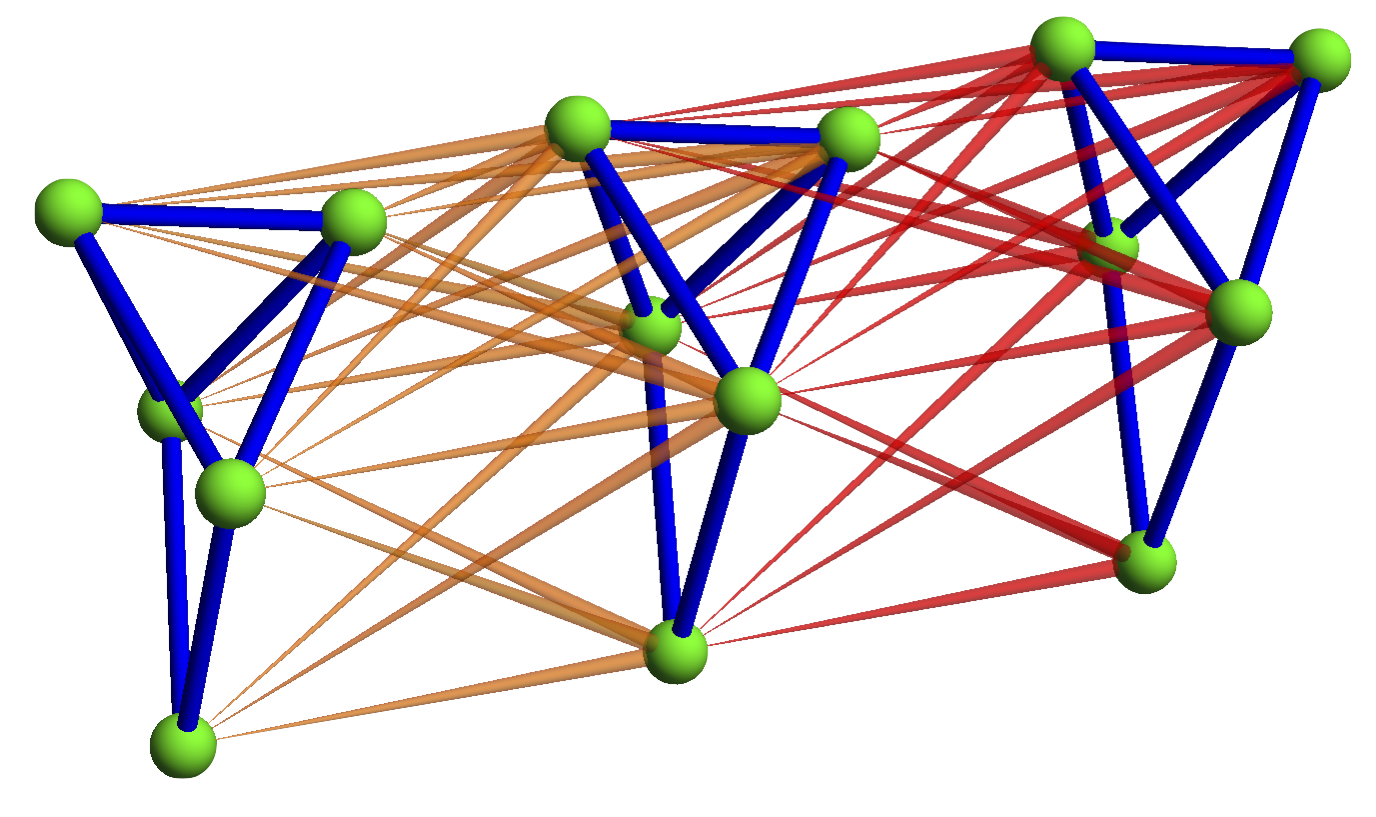
\includegraphics[width=\linewidth]{figs/gcnn.png}

Modified envelope~\citep{UnkeAP19}.

\begin{center}
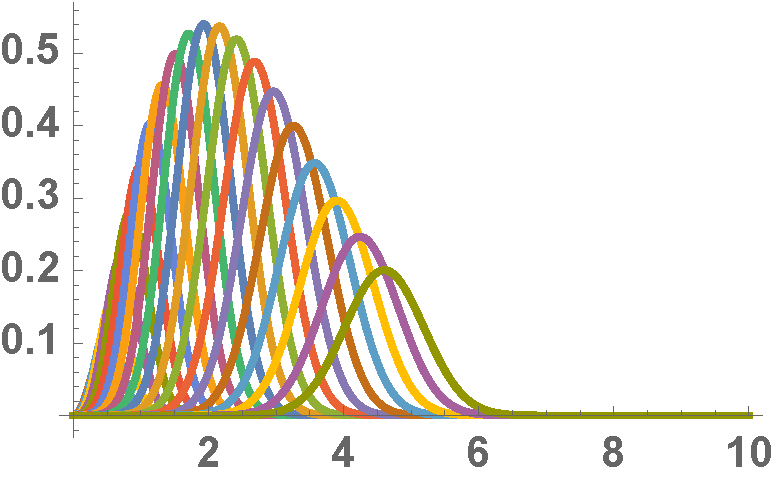
\includegraphics[width=0.6\linewidth]{figs/dist-features.pdf}
\end{center}

Schnet for electrons version 2:
\begin{equation}
\begin{aligned}
\mathbf x_i^{(0)}&:=\mathbf X_{\boldsymbol\theta} \\
\mathbf z_i^{(n,\pm)}&:=\sum\nolimits_{j\neq i}^\pm
  \mathbf w^{(n,\pm)}_{\boldsymbol\theta}
  \big(\mathbf e(\lvert\mathbf r_i-\mathbf r_j\rvert)\big)
  \odot\mathbf h_{\boldsymbol\theta}^{(n)}\big(\mathbf x_j^{(n)}\big) \\ 
\mathbf z_i^{(n,\mathrm n)}&:=\sum\nolimits_a
  \mathbf w_{\boldsymbol\theta}^{(n,\mathrm n)}
  \big(\mathbf e(\lvert\mathbf r_i-\mathbf R_a\rvert)\big)
  \odot\mathbf Y_{\boldsymbol\theta,a} \\
\mathbf x_i^{(n+1)}&:=\mathbf x_i^{(n)}
  +\sum\nolimits_\pm\mathbf g^{(n,\pm)}_{\boldsymbol\theta}
  \big(\mathbf z_i^{(n,\pm)}\big)
  +\mathbf g^{(n,\mathrm n)}_{\boldsymbol\theta}
  \big(\mathbf z_i^{(n,\mathrm n)}\big)
\end{aligned}
\end{equation}

Hartree--Fock from PySCF~\citep{SunWCMS18}.

\subsection{Sampling}

Standard Langevin Monte Carlo:
\begin{equation}
\mathbf r:=\mathbf r+\boldsymbol\nabla\ln\lvert\psi(\mathbf r)\rvert\tau+\boldsymbol\eta\sqrt\tau
\end{equation}

Quantum force $\equiv\boldsymbol\nabla\ln\lvert\psi\rvert\equiv\mathbf v$ changes too fast compared to step size $\mathbf v\tau$ close to nodes and nuclei.
Using techniques from \citet{UmrigarJCP93} with a simplification: around nuclei, step is limited in length such that the nucleus is never overshot.

Initial samples from Mulliken charges.

\subsection{Optimization}

\begin{equation}
\begin{gathered}
\mathcal L(\boldsymbol\theta)
  =\mathbb E_{\mathbf r\sim\lvert\psi'^2\rvert}
  \big[E_\text{loc}(\mathbf r;\boldsymbol\theta)\big] \\
\boldsymbol\nabla_{\boldsymbol\theta}\mathcal L(\boldsymbol\theta)
  =2\mathbb E_{\mathbf r\sim\lvert\psi'^2\rvert}\big[
    \big(E_\text{loc}(\mathbf r;\boldsymbol\theta)
    -\mathcal L(\boldsymbol\theta)\big)
    \boldsymbol\nabla_{\boldsymbol\theta}\ln\lvert\psi_{\boldsymbol\theta}\rvert
  \big]
\end{gathered}
\end{equation}

Gradient formula due to Hamiltonian being Hermitian~\citep{CeperleyPRB77}.

Stochastic gradient descent has been used in QMC previously~\citep{HarjuPRL97}.

Describe training protocol, hyperparameters.

\section{Results}

Code available at:

Reference results for first-row atoms:~\cite{SethJCP11}

\section{Discussion}

QMC small molecules:~\cite{NemecJCP10}.

Potential improvements:

Higher-order networks:~\cite{ThomasAC18}

Strong correlation with expressive Jastrow factors~\cite{GoetzJCTC17}

Universal wave functions, transferability.

Heavy atoms without pseudopotentials.

\subsubsection{FermiNet}

Differences:
\begin{itemize}
\item Pretrain w.r.t.\ HF vs.\ build in HF
\item Rotational invariance
\item Cusps built in vs learned
\item Network sizes
\item Architecture
\item K-FAC vs Adam for training
\item Langevin vs ordinary MC
\item training protocol
\end{itemize}

\subsubsection{Computational cost}

Nodes NP-hard~\citep{TroyerPRL05}.

Parallelism.

Laplace operator evaluation, scaling.

